% this file is called up by thesis.tex
% content in this file will be fed into the main document

%: ----------------------- introduction file header -----------------------
\chapter{Musiktherapeutische Stimmarbeit}
\label{chapter:musiktherapeutische_stimmarbeit}

\setlength{\epigraphwidth}{8.0cm}
\begin{spacing}{1.0}
\epigraph{Singen als Ausdruck von Gefühl, Gedanken und Identität, als Bewältigung und soziale Aktivität, die Fühlen und Denken synchronisiert und Gemeinschaftsgefühl, Nähe und Zugehörigkeitsgefühl erzeugt, ist ein Kommunikationsmedium, das von frühester Kindheit bis in die letzten Lebensphasen des Menschen eine besondere Rolle spielt.}{Heiner Gembris \autocite[12]{gembris2008}}
\end{spacing}
\ifpdf
    \graphicspath{{3_musiktherapeutische_stimmarbeit/figures/PNG/}{3_musiktherapeutische_stimmarbeit/figures/PDF/}{3_musiktherapeutische_stimmarbeit/figures/}}
\else
    \graphicspath{{3_musiktherapeutische_stimmarbeit/figures/EPS/}{3_musiktherapeutische_stimmarbeit/figures/}}
\fi
% ----------------------------------------------------------------------
%: ----------------------- introduction content -----------------------
% ----------------------------------------------------------------------
\lettrine{I}{n} diesem Zitat wird in knapper, jedoch prägnanter Form zusammengefasst, wie wichtig und wertvoll der stimmliche Ausdruck für den Menschen ist. In den folgenden Kapiteln soll das hier Skizzierte ausgeführt und -geweitet werden, um einen Eindruck von den Möglichkeiten der Stimmarbeit im musiktherapeutischen Kontext zu vermitteln.

Bevor im Folgenden selbstverständlich mit dem Begriff der "`Stimme"' umgegangen wird, scheint es sinnvoll, eine kleine Einführung in diese Thematik zu geben, um zum Einen die Komplexität der Funktionsweise unseres körpereigenen Instruments zu verstehen und um zum Anderen eine gemeinsame Grundlage für die Ausführungen in den daran anschließenden Kapiteln zu schaffen. 

Betrachtet man den gesamten Stimmapparat etwas genauer, so wird man feststellen können, dass seine Komplexität weit über das für das Sprechen Notwendige hinausgeht, welches nur einen kleinen Teil unserer Stimmorgane für seine Erzeugung benötigt \autocite[vgl.][38]{cramer1998}. Dies lässt sich evolutionär begründen, woraus auch ein Grundbedürfnis des Menschen zum gesanglichen Ausdruck abgeleitet werden kann.

Bevor die Menschheit Sprache entwickelte, war die lautliche und gesangliche Kommunikation vermutlich "`Gang und Gebe"'. "`Der Mensch hat sich früher singend – oder besser klingend – durchs Leben bewegt, denn mit Musik hatte seine Lautäußerung zunächst wenig zu tun. Stimme war Ausdruck der Lust, der Trauer, der Freude, des Hunger- und Sättigungsgefühls"' \autocite[8]{cramer1998}.

Auch zu Beginn des Lebens ist uns dieses musikalische, gesangliche Element in der Kommunikation mit dem Außen aber auch im eigenen Spiel geläufig. Der Säugling nimmt die Klänge um sich herum noch stärker in auf- und absteigenden Linien, rhythmischen Strukturen und plötzlich auftauchenden und schnell verschwindenden Hörerlebnissen wahr. Daniel Stern bezeichnet diese dynamischen Empfindungen als Vitalitätsaffekte. Diese sind verbunden mit körperlichen Vorgängen wie dem Durstig- oder Hungrigwerden, der Verdauung und dem Ausscheiden, Schmerz u.a. Er verwendet für die Beschreibung dieser auftauchenden Gefühlsregungen Begriffe wie "`verblassend"', "`abklingend"', "`sich hinziehend"', "`explosionsartig"' oder "`abschwellend"'.
So bedeutet Stimmäußerung beim Säugling ähnlich wie bei unseren frühen Vorfahren Ausdruck innerer Gefühls- und Bedürfnisregung \autocite[vgl.][83]{stern2007}. 

Wie man durch intrauterine Mikrofonaufnahmen herausgefunden hat, beginnt der Fetus wohl bereits während der Schwangerschaft im Fruchtwasser leise vor sich hin zu brabbeln (vgl. Decker-Voigt 2000: 282). Ab dem ersten Schrei kann auch die Umwelt an seinem klanglichen Ausdruck teilhaben. Um dem Säugling das Schlucken zu erleichtern und somit dem Verschlucken entgegenzuwirken, steht der Kehlkopf (Larynx) in den ersten drei Lebensmonaten noch etwas höher und senkt sich dann langsam ab. Von diesem Zeitpunkt an ist es ihm möglich, durch den gewonnenen Resonanzraum auch Laute entstehen zu lassen \autocite[vgl.][36]{cramer1998}. Dieser Resonanzraum wird auch Ansatz- oder Vokalrohr genannt und umfasst die Bereiche von Mund, Rachenraum (Pharynx) und Nasenhöhle. Bevor jedoch ein spezifisches Geräusch oder ein Klang hörbar wird, bekommt er seine erste Form im Kehlkopf. Dieser Prozess beginnt jedoch nicht erst mit dem Ausatmen, sondern bereits beim Einatmen. 

todo Grafik Kehlkopf Spornitz gescanntes Bild \ref{fig:kehlkopf} und \ref{fig:kehlkopf_vorne}

\begin{figure}
  \centering
  \subfigure[Kehlkopf von vorn]{
    \label{fig:kehlkopf_vorne}
    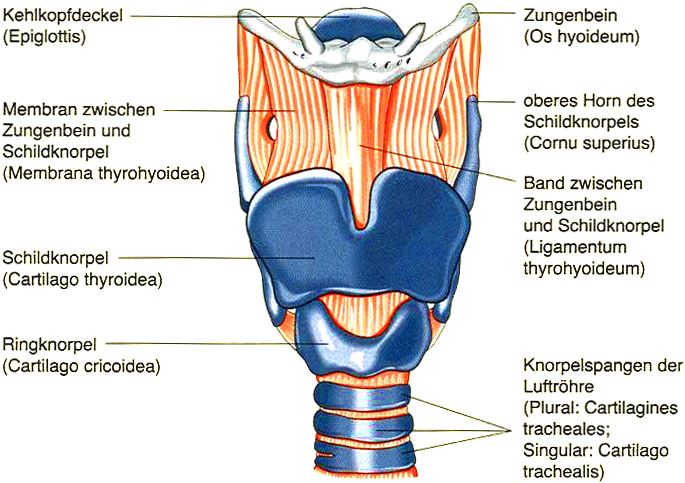
\includegraphics[width=0.47\textwidth]{kehlkopf_vorne}
  }
  \hfill
  \subfigure[Medianschnitt des Kehlkopfs sowie mittig gefensterte Region der Stimmbänder]{
    \label{fig:kehlkopf_seite}
    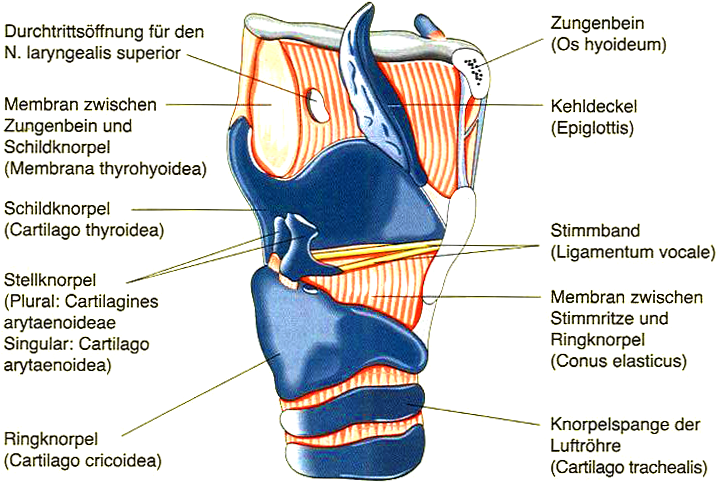
\includegraphics[width=0.47\textwidth]{kehlkopf_seite}
  }
  \caption[]{\subref{fig:kehlkopf_vorne} zeigt die Lagebeziehung von Kehlkopf und Zungenbein. Beide sind durch Membranen und Bänder miteinander verbunden. \subref{fig:kehlkopf_seite} Seitenansicht des Kehlkopfs, der Bereich rund um die Stimmbänder wurde in dieser Abbildung gefenstert (beide Abbildungen wurden \cite[271]{spornitz2010}, entnommen)}
  \label{fig:kehlkopf}
\end{figure}

Die Stimmerzeugung basiert auf dem Zusammenspiel zwischen Körper, Atem und Stimmapparat (Kehlkopf und Ansatzrohr), wobei der ganze Körper als Resonanzkörper fungiert. Der Kehlkopf gilt als das komplexeste motorische System unseres Körpers und ist für die Stimmentstehung primär verantwortlich. Jedoch bedarf er für diesen Prozess des gesamten Körpers. Am Sprechvorgang sind laut Cramer "`mehr als 100 Muskeln von Kehlkopf, Zunge, Rachen, Kiefer und Lippen beteiligt. Dazu kommen noch die Muskelsysteme der Mimik und der Atemgebung"' \autocite[40]{cramer1998}. So kann man sich vorstellen wie hochkomplex der Prozess der Feineinstellung und -abstimmung dieser gesamten Muskeln und beteiligten Nervenstränge ist. 

Atem und Kehlkopffunktionen sind abhängig von dem Zusammenwirken und dem Spannungszustand der Muskeln. Haben wir beispielsweise aufgrund eines plötzlich auftretenden, angstauslösenden Ereignisses einen erhöhten Körpertonus, so wird dies zwangsweise dazu führen, dass wir nicht mehr entspannt ein- und ausatmen, da sich die erhöhte Anspannung auch auf unsere Atemmuskulatur, insbesondere auf das Zwerchfell als wichtigstem und größtem Atemmuskel, überträgt. 

Bevor es zu einer stimmlichen Äußerung kommt, bedarf es des Einfließens der Luft in die unteren Atemwege, die Lunge. Die Atmung als lebensnotwendiger Prozess wird über das Vegetativum gesteuert, das heißt, sie erfolgt für normal nicht willentlich gelenkt. Allerdings haben wir mit einem weiteren Atemzentrum in der Großhirnrinde die Möglichkeit, Sprach- und Denkaktivitäten mit dem Atem zu verbinden sowie diesen bewusst zu steuern \autocite[vgl.][2]{ehrmann2004}. 

Am Atemvorgang ist die gesamte Atemhilfsmuskulatur beteiligt. Diese spannt sich von den Schultern über die Zwischenrippenmuskeln bis hin zu unserem Hauptatemmuskel, dem Zwerchfell (siehe Abbildung \ref{fig:zwerchfell}). Dieses trennt den Brustkorb von den Bauchorganen und ist für die Atmung von großer Bedeutung. Bei der Einatmung senkt es sich durch das Füllen der Lungen mit Luft nach unten und massiert so, jedenfalls bei der richtigen Bauchatmung, die Organe. Beim Ausatmen schlafft es wieder zusammen und gibt den Organen Raum (Abbildung \ref{fig:zwerchfell_atembewegung}). Es unterstützt dabei die Lunge beim Ausströmen-lassen der Luft. Steht das Zwerchfell jedoch unter besonderer Anspannung, wie dies oftmals aufgrund einer veränderten Atmung bei COPD-Patienten der Fall ist, so hat dies im Umkehrschluss auch Auswirkungen auf eine ansonsten entspannte, fließende Atmung. 

\begin{figure}
  \centering
  \subfigure[Das Zwerchfell]{
    \label{fig:zwerchfell}
    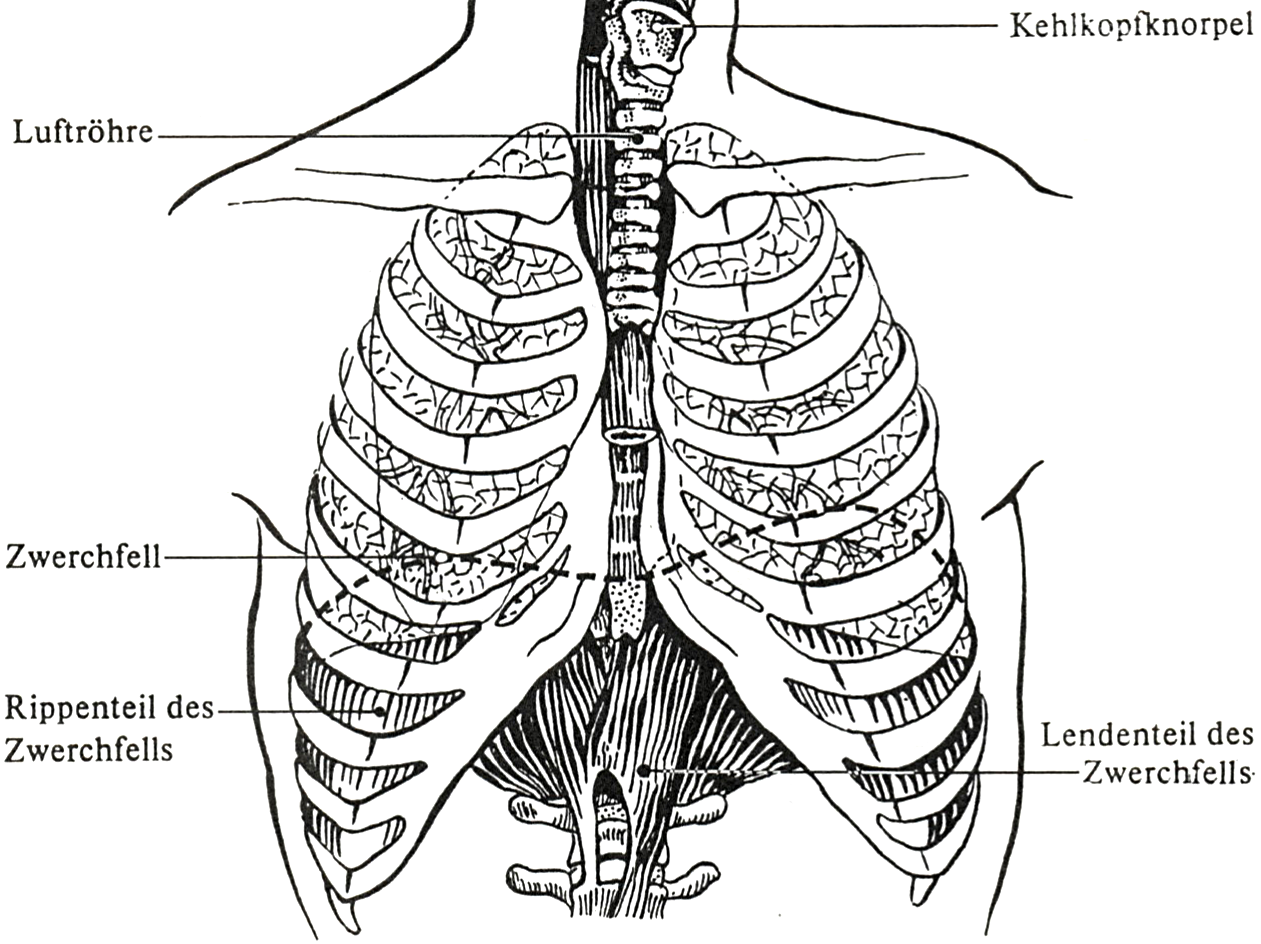
\includegraphics[width=0.47\textwidth]{zwerchfell}
  }
  \hfill
  \subfigure[Zwerchfellstellung bei In- und Exspiration]{
    \label{fig:zwerchfell_atembewegung}
    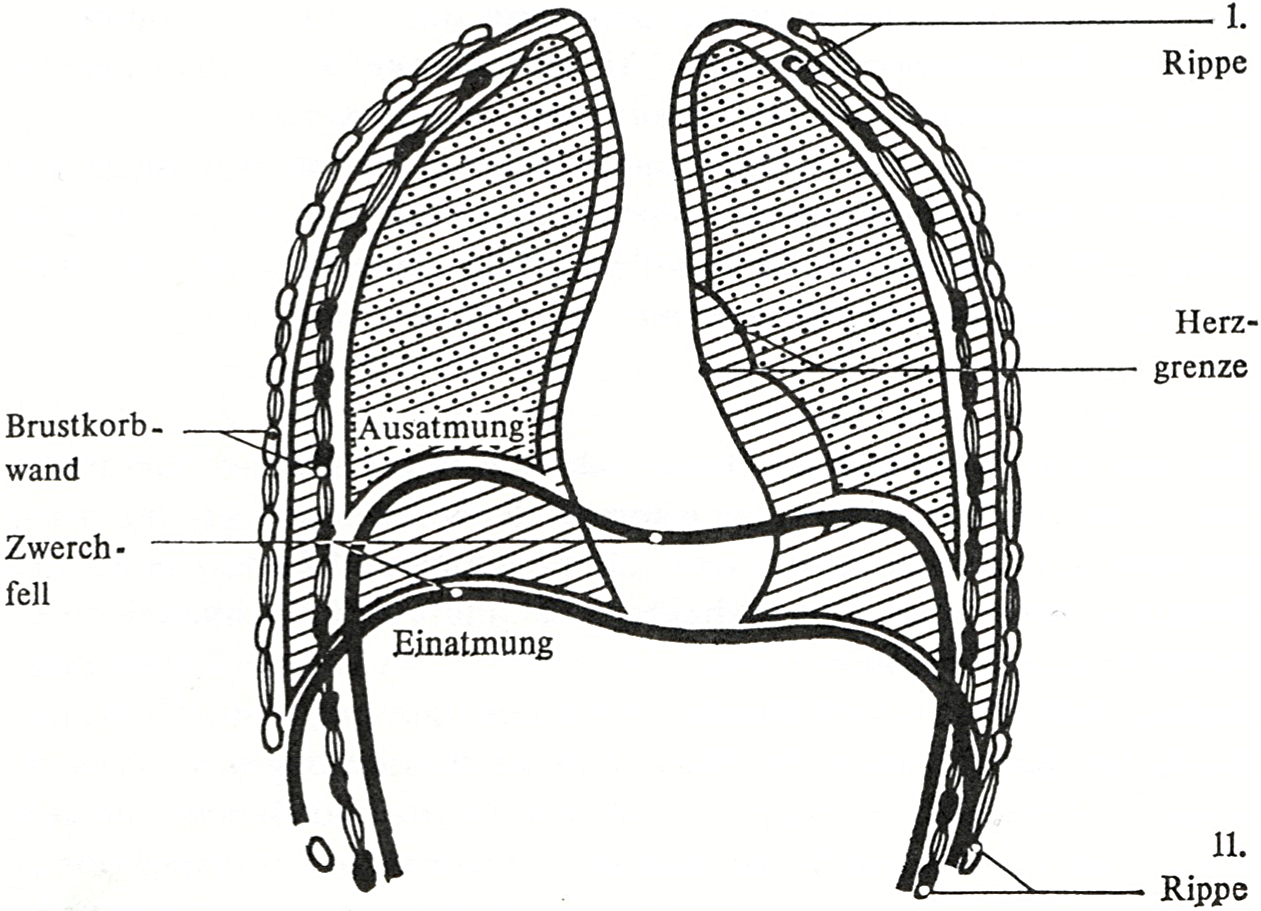
\includegraphics[width=0.47\textwidth]{zwerchfell_atembewegung}
  }
  \caption[]{Abbildung \subref{fig:zwerchfell} zeigt das Zwerchfell, den wichtigsten Atemmuskel, von vorn. Es trennt die Brusthöhle von der Bauchhöhle (entnommen aus \cite[48]{seidner2010}), Abbildung \subref{fig:zwerchfell_atembewegung} zeigt schematisch die veränderte Zwerchfellstellung beim Atemvorgang (entnommen aus \cite[53]{seidner2010})}
  \label{fig:zwerchfell_gesamt}
\end{figure}

Die Atemluft strömt beim Einatmen durch die sich im Kehlkopf befindenden und in Dreicksform geöffneten Stimmlippen in die darunter befindliche Luftröhre. Kommt es nun zu einer stimmlichen Äußerung, schließt sich im ersten Schritt die Glottis, auch Stimmritze genannt, nach vollendetem Einatmen (siehe Abbildung \ref{fig:stimmlippen}). Anschließend wird durch das nun folgende Ausatmen ein Überdruck auf die geschlossenen Stimmlippen erzeugt, welcher diese in Schwingung versetzt. Dieser "`streng periodische Schwingungsvorgang"' \autocite[481]{rittner2009a} sei laut Rittner abhängig von Elastizität, Masse, Kontur, Spannung und Stellung der Stimmlippen \autocite[vgl.][481]{rittner2009a}.

\begin{figure}
  \centering
  \subfigure[Aufsicht auf die Glottis bei normaler Ruheatmung]{
    \label{fig:stimmlippen_offen}
    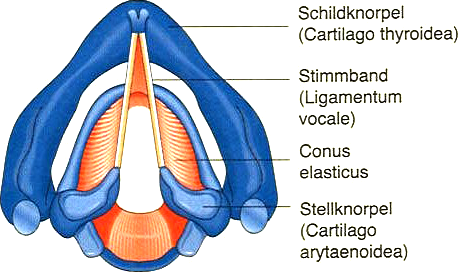
\includegraphics[height=5cm]{stimmlippen_offen}
  }
  \hfill
  \subfigure[Aufsicht auf die Glottis bei Stimmbildung (Phonation)]{
    \label{fig:stimmlippen_phonationsstellung}
    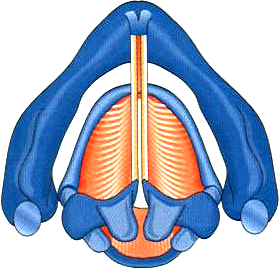
\includegraphics[height=5cm]{stimmlippen_phonationsstellung}
  }
  \caption[]{Von der Innenseite des Schildknorpels verläuft das Stimmband an die Stellknorpel. Das Stimmband und der Ringknorpel sind durch eine Membran, die die unteren Luftwege gegen das Stimmband abschließt, verbunden (entnommen aus \cite[271]{spornitz2010}).}
  \label{fig:stimmlippen}
\end{figure}

Durch die Glottis entweichen die Luftmoleküle in dosierter und schwingender Form, erhalten im Ansatzrohr ihre ganz eigene klangliche Färbung und können nun von der Umwelt gehört werden. Die Stimme erhält ihre besondere Klangfarbe, welche keiner anderen Stimme auf der Welt gleicht, durch ihre ganz eigenen Obertöne. So wird sich beispielsweise dieses Wissen in der Kriminalistik zu Nutzen gemacht. Denn unabhängig von der wechselnden Stimmungslage kann der individuelle Stimmklang auch als "`klanglicher Fingerabdruck"' \autocite[482]{rittner2009a} mithilfe von Spracherkennungssystemen entschlüsselt werden. 

In den folgenden Kapiteln wird neben einer kurzen geschichtlichen Darstellung sowohl auf den Einsatz der Singstimme im musiktherapeutischen Kontext als auch auf die Wirkung des Singens auf Körper und Psyche eingegangen.

\section{Geschichtliche Einführung in das Thema}
Zu Beginn der weiteren Ausführungen in diesem Kapitel sollte der Blick auf den Gebrauch der Singstimme in der Gesellschaft gewendet werden, um ein klareres Gesamtbild dieses Themas entstehen lassen zu können.

Während das Singen in unserer Großelterngeneration noch weit verbreitet war, man beachte unseren großen Umfang an deutschem Liedgut, so hat die nationalsozialistisch geprägte Zeit der 30er und 40er Jahre einen Keil in diesen selbstverständlichen Gebrauch der Singstimme in Gemeinschaft getrieben.
Die Verschandelung deutschen Liedguts mit nationalsozialistischem Gedankengut und der Einsatz desgleichen für propagandistische Zwecke wie im Besonderen in der Jugendmusikbewegung der damaligen Zeit geschehen, führte u.a. zu "`der späteren Voreingenommenheit gegenüber gemeinsamem Singen im Allgemeinen und gegenüber dem deutschen Volkslied im Speziellen"' \autocite[9]{wolf2012}.

Hinzu kommt seitdem die Entwicklung neuer Medien und die Möglichkeit eines geöffneten Zugangs zu diesen. Laut Wolf hat dies großen Einfluss auf "`die Entwicklung hin zu einer Vereinzelung der Menschen und hin zu einer Veränderung des menschlichen Alltagverhaltens"' \autocite[10]{wolf2012}. Dadurch ließ die Notwendigkeit der gemeinschaftlichen Freizeitgestaltung, welche in früheren Zeiten oftmals das gemeinsame Singen beinhaltete, nach. Nur an vereinzelten Schauplätzen wie z.B. im Gottesdienst, im Stadion, bei den Pfadfindern oder in Chören wird das gemeinschaftliche Singen und/oder Grölen noch aktiv praktiziert.

In der Musiktherapie war der Einsatz der Singstimme ebenfalls lange Zeit negativ konnotiert und wurde "`[\ldots] als "`Konflikt vermeidende Technik"' in dem heilpädagogisch orientierten Bereich der Kindermusiktherapie oder dem palliativ orientierten Feld der Geriatrie verortet"' \autocite[10]{wolf2012}. So war das Singen von Liedern im Rahmen einer "`psychotherapeutisch orientierten Musiktherapie"' lange Zeit ausgeklammert. Zudem wurde die Stimme zum klanglichen Ausdruck kaum genutzt, da man einen zu großen Widerstand seitens der Patienten erwartete (siehe weiter unten in diesem Kapitel). 

Durch den sich in den letzten Jahren vollziehenden Paradigmenwechsel in der psychotherapeutischen Behandlung im Allgemeinen und der Musiktherapeutischen im Speziellen von einem eher konfliktzentrierten Ansatz und dem Konzept der Katharsis hin zu einem eher ressourcenorientierten und stabilisierenden Arbeiten veränderte sich auch die Einstellung gegenüber dem Singen\autocite[vgl.][11]{wolf2012}. Einer kleinen Forschergruppe aus Musiktherapeuten und -pädagogen, aber auch bekannten Ärzten (wie z.B. Dr. Gerald Hüther, Dr. Manfred Spitzer u.a.) ist es zu verdanken, dass wir heute mehr über die Wirkung des Singens auf Körper, Geist und Seele wissen. Sie waren es, die zu einer Etablierung von Singgruppenarbeit primär beigetragen haben. Im klinischen Bereich hat sich insbesondere der Musiktherapeut Wolfgang Bossinger verdient gemacht und eine mittlerweile über Deutschland verbreitete Initiative, "`Singende Krankenhäuser"', ins Leben gerufen. Aber auch Sabine Rittner und Karl Adamek haben zu einem großen Erkenntnisgewinn und möglichen Vorgehensweisen in diesem Bereich verholfen.

\section{Einsatz der (Sing-)Stimme im musiktherapeutischen Kontext}

Heute wird die (Sing-)Stimme im psychotherapeutischen Kontext in unterschiedlicher Art und Weise eingesetzt, genutzt und betrachtet. Sabine Rittner \autocite[vgl.][204 ff.]{rittner2008} hat diese Bereiche kategorisiert, um ihre Komplexität zu entzerren. Diese insgesamt acht Kategorien fließen zum Teil in die folgenden Ausführungen ein: 
Stimme als\ldots
\begin{enumerate}
\item Medium der verbalen und nonverbalen Beziehungsgestaltung
\item Methode in der körperorientierten Musikpsychotherapie
\item Diagnostikum im therapeutischen Gespräch
\item Indikator für die therapeutische Übertragung- und Gegenübertragung
\item Symptom
\item Ausdrucksmittel
\item Selbstheilungs-Mittel
\item Medium zur Tranceinduktion
\end{enumerate}

Bereits im Mutterleib beginnt der Beziehungsaufbau zwischen Mutter und Kind über stimmliche Äußerung. Ab der 19.-24. Schwangerschaftswoche kann der Fötus seine Umwelt auditiv wahrnehmen und auf sie reagieren \autocite[vgl.][110]{deckervoigt2008}. Die Stimme der Mutter tritt dabei in den Vordergrund. Wie man durch Untersuchungen kurz nach der Geburt festgestellt hat, können Säuglinge die Stimme ihrer Mutter von der anderer Personen unterscheiden \autocite [vgl.][22f]{noecker-ribeaupierre2004}. 

Die stimmliche Äußerung ist für die Entwicklung des Kindes von besonderer Bedeutung: durch Abstimmungsprozesse mit den primären Bezugspersonen auf unterschiedlichen sensorischen Ebenen, insbesondere durch stimmliche Interaktion, lernt es, die Welt und sich über die so genannte amodale Wahrnehmung zu begreifen. Gerade in dieser Zeit wird deutlich, welche Bedeutung die Stimme im Hinblick auf die Mitteilung der eigenen emotionalen Gestimmtheit hat, wie sich Beziehung ohne Worte aber dennoch durch stimmlichen Ausdruck gestalten lässt. Insbesondere durch den Einsatz von Vokalen kann diese "`emotionale Tönung"' \autocite[205]{rittner2008} deutlich werden, wie weiter unten näher erläutert wird.

Rittner \autocite [vgl.][106f.]{rittner1990} betont zudem die therapeutische Relevanz der Polaritäten, die sich im Schreien und Lallen des Säuglings äußern. Mit dem ersten Schrei tritt der Säugling zum ersten Mal geräuschvoll mit seiner neuen, doch zugleich auch bekannten Umwelt in Kontakt und entlädt dabei die zuvor im ersten Einatem aufgebaute Anspannung. Diese Form der Kontaktaufnahme mit der Außenwelt differenziere sich, so Rittner, in den darauffolgenden Wochen immer mehr zu einem "`gerichteten Appell"' in Bezug auf die Befriedigung der Grundbedürfnisse. Im Lallen hingegen zeige der Säugling aus einer befriedigten Grundstimmung heraus eine "`lustbetonte, nach innen gerichtete, autoerotisch-regressive Handlung"', die oftmals unterbrochen wird, sobald beispielsweise im Außen Geräusche auftreten oder eine Person das Zimmer betritt und ihn so aus seiner Versunkenheit herauszieht. 
Die o.g. Polaritäten können aus diesen beiden Handlungen heraus folgendermaßen beschrieben werden: 

\begin{quote}
\onehalfspacing
"`die Verbindung zwischen Innenraum und Außenraum, zwischen Regression, dem wohligen Sich-Einhüllen, und Progression, in der sich lebenserhaltende aggressive Anteile artikulieren"' \autocite[106f.]{rittner1990}. 
\end{quote}

Diese Aspekte sind wesentlich für die Gestaltung und die Arbeit im Rahmen einer therapeutischen Beziehung. Mithilfe musiktherapeutischer Stimmarbeit ist es uns somit möglich, in sehr direkter Form an diese sehr frühen Erfahrungswelten anzuknüpfen und an einer Ausbalancierung der o.g. Polaritäten zu arbeiten. 

Allerdings gilt es dabei u.a. zu beachten, dass der Mensch im Laufe seiner Entwicklung Hemmungsmechanismen ausbildet, welche auf die Sauberkeitserziehung sowie auf Sozialisationsprozesse zurückzuführen sind. Diese Mechanismen lassen sich gliedern in "`Scham- und Peinlichkeitsgefühle als auch (in) psychische Instanzen, die das Gewissen und Schuldgefühle auslösen"' \autocite [106f.]{rittner1990}. 

Durch das Singen kommen wir, wie bereits zuvor dargelegt, schnell in Kontakt mit unserer primär unbewussten Gefühlswelt. Aufgrund der Nähe zu "`frühkindlichen Gefühlszuständen vor der Schamhemmung"' (\cite{klausmeier1978} zitiert in \cite[107]{rittner1990}) und damit einem sehr intensiven emotionalen Erleben kann der unvorbereitete Einsatz der Singstimme überflutend und angstauslösend hinsichtlich des ungewollten Zeigens von u.a. abgewehrten Selbstanteilen wirken. 

Da das Thema Scham m.E. wichtig ist für die Arbeit mit der Stimme im musiktherapeutischen Rahmen und bereits am Anfang dieses Kapitels in Wolfs Aussage zu Widerständen in diesem Kontext anklingt, soll an dieser Stelle darauf eingegangen werden.

\subsection{Scham und Stimme}
\label{scham_und_stimme}
Zunächst eine kurze Erläuterung des Begriffs. Unter dem Titel "`Scham. Lautloses Tönen"' erschien 2012 ein Themenheft der Musiktherapeutischen Umschau (MU). Hierin beschrieb Tilman Weber in knapper Form und aus unterschiedlichen theoretischen Perspektiven die "`Scham"' folgendermaßen:

\begin{quote}
\onehalfspacing
"`Vielleicht kann man sagen, dass Scham aus triebpsychologischer Sicht einem typischen Es - Überich - Konflikt entspringt, aus objektpsychologischer Sicht der Diskrepanz zwischen Individuum und Gesellschaft und aus ichpsychologischer Sicht der Differenz zwischen Anspruch und Vermögen"' \autocite[215]{weber2012}. 
\end{quote}

Tiedemann, tiefenpsychologischer und analytischer Psychotherapeut und Forscher, beschreibt Scham als einen Vorgang, in dem "`das Subjekt eine Infragestellung und Bedrohung der sozialen Wertschätzung, Akzeptanz und Anerkennung"' \autocite[219]{tiedemann2012} erlebt. Daher tritt sie meist in solchen Situationen auf, in denen ein "`Mensch etwas Intimes preisgibt"' \autocite[219]{tiedemann2012}. 

Die Stimme ist das intimste körpereigene Instrument des Menschen. Jede stimmliche Äußerung gibt ein Stück unserer individuellen Ge-stimmt-heit preis. An unterschiedlichen Stellen in der hierzu relevanten Literatur wurde immer wieder darauf hingewiesen, dass eine stimmliche Maskierung des eigenen affektiven Zustandes nicht möglich ist (\cite[vgl.][279]{deckervoigt2000} und \cite[vgl.][481]{rittner2009a}). Je nach Stellung der Stimmknörpelchen und des Tonus der über 100 an der stimmlichen Äußerung beteiligten Muskeln \autocite[vgl.][40]{cramer1998} gestaltet sich das nach außen Dringende. Denn jegliches Zurückhalten oder Verdecken von aufkeimenden Emotionen führt zu Störungen der Feinabstimmung innerhalb des Stimmapparates. Dies kann zu Muskelverspannungen führen, die wiederum in der erklingenden Stimme durch einen harten Stimmansatz, Verhauchen der Stimme durch nicht zu Klang gewordene herausströmende Luft, eine höhere oder tiefere Stimmfrequenz u.a. hörbar werden \autocite[vgl.][279]{deckervoigt2000}. 

Laut Rittner vernehmen wir die "`emotionale Tönung"' der Person durch die Prosodie [=das, was dazu singt). Insbesondere durch den Klang der Vokale, welche physikalisch betrachtet als Klangträger gleichmäßige Schwingungsmuster, Konsonanten hingegen als Geräuschträger ungleichmäßige Schwingungswellen erzeugen, erfahren wir im Sinne der o.g. physiologischen Vorgänge etwas über die Gestimmtheit unseres Gegenübers. Dabei kommt dem Singen eine besondere Rolle zu: "`Singen unterscheidet sich vom Sprechen dadurch, dass der klanglich-nonverbale Schwingungsanteil der emotionalen Botschaft durch die Verlängerung der Vokale im ausgedehnten Ausatem deutlich in den Vordergrund tritt"' \autocite[205]{rittner2008}.

Wie unmittelbar stimmliche Äußerung auf unsere Umwelt wirkt und wie jeder Einzelne sogar körperlich für diese so spürbar wird, fasst Rittner in dem Begriff der "`klanglich-organismischen-Resonanz"' zusammen, wobei sich dieses Phänomen auch bereits in dem gesangstechnischen Begriff des "`funktionellen Nachvollzugs"' finden lässt. Wir kennen dieses Phänomen aus unterschiedlichen Kontexten, wie z.B. in einem Wartezimmer beim Arzt, wenn jemand hustet und bei einem selbst im Hals etwas anfängt zu kratzen oder aber der Räuspereffekt in einem Konzert. Dies lässt sich auf folgende Vorgänge beziehen: wie bereits weiter oben beschrieben, ist unser Kehlkopf über einen Ast des nervus vagus, dem s.g. nervus laryngeus inferior, mit unserem Vegetativum verbunden \autocite[vgl.][106]{rittner1990}. Stimmliche Äußerungen eines Gegenübers nehmen wir unmittelbar "`durch unwillkürliche Übertragung neuromuskulärer Vorgänge und Atemfrequenzen"' \autocite[482]{rittner2009a} körperlich auf; dabei ist die Intensität der Übertragung situativ unterschiedlich. Wie Neurowissenschaftler feststellten, ist für diesen Prozess nicht nur ein stimmlich-vegetativer Zusammenhang verantwortlich, sondern auch die Aktivität s.g. Spiegelneuronen im Gehirn. Forscher haben sogar eine erstaunliche Schnelligkeit dieses Vorgangs gezeigt: ein Entschlüsseln der emotionalen Gestimmtheit des Sprechers geschieht in 150 Millisekunden\autocite[vgl.][482]{rittner2009a}.

Die vorherigen Ausführungen machen deutlich, dass es sich bei der stimmlich-gesanglichen Äußerung um ein sehr unmittelbares und intimes Zeigen der emotionalen Verfassung handelt. Die stimmliche Äußerung ist direkter als das Spielen eines Musikinstruments, welches bereits räumlich von uns getrennt ist und einen "`strukturellen Schutz"' \autocite[292]{deckervoigt2000} bietet im Sinne eines sich dahinter Verstecken-Könnens. Wenn wir also im musiktherapeutischen Kontext mit der Singstimme arbeiten, sollten wir uns dieser unmittelbaren Verbindung bewusst sein. Denn das Singen, vorallem in der Improvisation, welche häufig mit der Sorge um Kontrollverlust verbunden ist, kann als "`zu starker emotionaler Ausdruck abgewehrt und blockiert werden"' \autocite[485]{rittner2009a}. Um jedoch der Abwehr aus Scham entgegenzuwirken, sei es laut Rittner wichtig, stimmliche Interventionen im Verlauf der musiktherapeutischen Behandlung methodisch anzubahnen. So könne beispielsweise mit bekannten, durchkomponierten Liedern, Melodien und Rhythmen begonnen werden, um sich der ursprünglichen stimmlichen, improvisierenden Äußerung, wie sie zu Beginn des Lebens wertfrei bestand, zu nähern. 

\subsection{Diagnostische Überlegungen}
\label{subsection:diagnostische_ueberlegungen}
Im Rahmen der Diagnostik gibt die Stimme des Patienten bereits wichtige Hinweise auf dessen aktuelle Befindlichkeit sowie seine Stimmung. Durch aufmerksames Hinhören kann erspürt werden, ob das Gesagte in sich "`stimmig"', sprich kongruent ist. Zudem gibt die Stimme bereits Auskunft über den biografischen Hintergrund der sich äußernden Person, denn sie hat sich mit unseren über die Zeit gesammelten Lebenserfahrungen weiterentwickelt und diese in sich aufgesogen. So gilt die Stimme unter Experten als "`Klingendes Hologramm der Persönlichkeit"' \autocite[222]{adamek1999}, "`lauthafte Biographie"' \autocite{gundermann1994} und bei Rittner erfahren wir über den Klang der Stimme etwas über die "`leib-seelische Gewordenheit"' \autocite[211]{rittner2008} des Menschen.
Dabei scheint jedoch nicht so sehr der Inhalt des Gesagten aufschlussreich, sondern vielmehr der 

\begin{quote}
\onehalfspacing
"`Klang der Stimme (Klangspektrum, Modulation, Lautstärkeänderungen, Stimmsitz, Vokaleinsatz etc.), die Sprechweise (Artikulation, Phrasierung, Pausensetzung etc.) und die Atmung (Atemfrequenz, Atemtiefe, hörbares Einatmen, Sitz des Atemraumes im Körper etc.)"' als auch "`die Art der Gestaltung von Sprechpausen, Abbrüchen, Momenten des Innehaltens, Verzögerungen u.ä."' \autocite[210]{rittner2008}. 
\end{quote}

Diese stillen Momente intensivieren jedoch oftmals das atmosphärische Wahrnehmen und können zu einem tieferen Verstehen ohne Ablenkung führen. 
Gerade in Momenten der Inkongruenz von Semantik, Prosodie, Mimik und Gestik wurde festgestellt, dass der Zuhörer sich in diesem Falle weniger auf den Inhalt des Gesprochenen seines Gegenübers bezieht, sondern in einen visuell-auditiven Modus wechselt, in welchem die Semantik in den Hintergrund rückt \autocite [vgl.][206f.]{rittner2008}.

\subsection{Methodische Möglichkeiten der Stimmarbeit}
\label{methodische_moeglichkeiten_der_stimmarbeit}

In der musikterapeutischen Stimmarbeit haben wir verschiedene methodische Möglichkeiten des Vorgehens. In der von Sabine Rittner entwickelten "`körperorientierten Psychotherapie"' dient die Stimme im therapeutischen Prozess als Arbeitsmittel. Je nach Bedarf werden hier unterschiedliche Interventionen auf übungs-, erlebnis- oder konfliktzentrierter Ebene eingesetzt. In diesem Kontext hat die Stimme unterschiedliche Einsatzbereiche: "`als körperorientierte psychotherapeutische Methode, als Weg zur Wahrnehmungsschulung, als Mittel zur Ausdrucksförderung, als Agens zur Bearbeitung unbewussten Konfliktmaterials und als Medium zur emotionalen und physischen Ressourcenaktivierung"' \autocite[58]{rittner2012}. Neben diesen Gesichtspunkten bedeutet Singen im therapeutischen Setting Schulung der Körperwahrnehmung, Beobachtung und Veränderung der eigenen Atmung sowie Konzentration auf Selbst- und Fremdwahrnehmung und Kontakt.
Einige dieser Aspekte sollen anschließend in Kurzform dargestellt werden.

\emph{Das therapeutische Gespräch} stellt einen wichtigen Teil unserer Arbeit dar. In der psychotherapeutischen Arbeit mit Patienten dient die Stimme als Medium der verbalen und nonverbalen Kommunikation und ist somit wesentlich an der Beziehungsgestaltung beteiligt. Laut Rittner bestehe der größte zeitliche Anteil einer musiktherapeutischen Sitzung aus dem therapeutischen Gespräch. Dementsprechend erscheint es auch wichtig, sich über die eigene Sprechstimme bewusst zu sein. Wie gestalte ich selbst das Gespräch? Durch die Art und Weise, wie ich meine Stimme forme, das Sprechtempo aufnehme oder verändere, pausiere oder mitatme und mitschwinge, nehme ich auf die Gesprächsgestaltung Einfluss. Auch die Form der gesendeten Botschaften, ob Pacing (folgend) oder Leading (leitenden), scheint an diesem Punkt erwähnenswert. Meist vermitteln sich diese Botschaften nonverbal. Dabei ist oftmals der Anteil an Pacing-Botschaften zu Beginn eines Therapieprozesses aufgrund des Aufbaus einer sicheren und vertrauensvollen therapeutischen Beziehung noch höher (ca. 70-80\%). Diese Tendenz wird sich im Verlauf der Therapie jedoch immer mehr zugunsten des Leadings umkehren, maximal jedoch einen Anteil von 50\% erreichen \autocite[vgl.][208]{rittner2008}.

\emph{Vokalimprovisationen} sind eine sehr spielerische Möglichkeit, die Stimme in die musiktherapeutische Arbeit einzubeziehen. Sie gilt als der "`Einsatz des gesamten Ausdrucksspektrums stimmhafter wie stimmloser Äußerungen, meist im Schutz einer Gruppe mit oder ohne Themenvorgabe"' \autocite[108]{rittner1990}. Dabei sei sie stets gebunden an persönliche, situative, musikalisch oder symbolische Inhalte und verfolge therapeutische, pädagogische oder musikalisch-künstlerische Ziele \autocite[vgl.][109]{rittner1990}. 

Stimmimprovisationen können frei oder themenfokussiert gestaltet werden. In der freien Improvisation begibt sich der Musizierende ohne Regeln in einer offenen Haltung in ein sich ihm eröffnendes Spektrum an Empfindungsqualitäten und Erfahrungswelten. Gerade im Schutz einer Gruppe wird es möglich, sich stimmlich auszuprobieren, tabuisierte Geräusche und Klänge von sich zu geben, ohne sich dafür schämen zu müssen. 
Das Singen in diesem Rahmen fördert so eine Vielfalt an Ausdrucksmöglichkeiten und lässt unterschiedliche Stimmungsnuancen hörbar werden.

In der stimmlichen Improvisation können Körpergeräusche, stimmlose und stimmhafte (wie z.B. beim Summen) Konsonanten, Vokale in Form von Einzeltönen, kurzen Tonfolgen oder Melodien aber auch sprachliche Äußerungen eingesetzt werden \autocite[vgl.][109]{rittner1990}. Bossinger stellt in diesem Zusammenhang heraus, dass durch den Prozess in dieser Arbeit "`die ursprüngliche Lebendigkeit und Ausdrucksfähigkeit des inneren \emph{musikalischen} Kindes in uns wiederentdeckt und erlebt werden"' \autocite[272]{bossinger2006} kann.

Die themenfokussierte Improvisation kann Hemmungen entgegenwirken und bietet dennoch die Möglichkeit zum vertieften Einsteigen in den individuellen stimmlichen Ausdruck. Beispielsweise kann gemeinsam über eine oder mehrere bestimmte Emotionen improvisiert werden. Bei Bossinger findet sich für diese Improvisationsidee der Titel "`Gefühls-Cocktail"'. Durch diese Form des Improvisierens gewännen die SängerInnen, laut Bossinger, wieder mehr spontanen und freien Zugang zu ihren Gefühlen und Ausdrucksmöglichkeiten \autocite[vgl.][273]{bossinger2006}. Eine weitere Form stellt das Improvisieren über Metaphern, Bilder, Geschichten evtl. sogar konkrete Situationen dar. So kann die eigene Phantasie und Wahrnehmung angeregt und erweitert werden. Aber auch über Worte, Gedichte oder Affirmationen lässt sich improvisieren. Diese Formen sollten jedoch stets an die Bedürfnisse der Gruppe oder des Einzelnen angepasst sein.

\emph{Das Tönen}, auch Toning genannt, ist eine Form der Stimmimprovisation, in dem ein schöpferischer, kreativer Prozess im Vordergrund steht. Aus dem Fluss des Atems treten allmählich Geräusche und Klänge hervor. Mithilfe des Tonings können wir stärker in Kontakt mit unserer Stimme, unserer Atmung und unserem Körper gehen und in unsere ganz eigene Gefühlswelt eintauchen. Zu Beginn empfiehlt es sich, im Stehen zu tönen, da der Atem in der Aufrechte leichter fließen kann. Ein fester Stand, mit lockeren Knien und Becken und aufrechter Haltung erleichtert das reflexive Atmen und gibt zudem Kraft durch einen festen Untergrund. Außerdem gibt es verschiedene Möglichkeiten, das Tönen in der Gruppe zu gestalten. Hier sind Formen stehend, sitzend oder liegend im Kreis oder im Raum verteilt, sowohl zu- als auch abgewandt denkbar. Eine weitere Variante stellt das so genannte Besungen werden dar. Hierbei handelt es sich um einen Vorgang, der sehr an die frühen Erfahrungen erinnert, welche wir im Rahmen einer positiv besetzten Bindungsbeziehung gemacht haben. Die Teilnehmer stimmen sich auf die zu Besingenden ein und lassen ihre Stimmen in feinfühliger Weise erklingen. Dies hat Bossinger zu Folge "`eine tiefgreifende Wirkung, sowohl auf Sänger wie auch auf Besungene und initiiert Tranceprozesse"' \autocite[275]{bossinger2006}. Eine weitere Form stellt das "`Tönen im achtsamen Körperkontakt"' \autocite[208]{rittner2008} dar. Dies ist eine Methode aus der musiktherapeutischen Körperarbeit, welche "`sowohl zur effektiven Selbstbehandlung für die Patienten, als auch zur Behandlung durch Hände und Stimme der Therapeutin/des Therapeuten eingesetzt werden"' \autocite[208]{rittner2008}. Dabei liegt der Fokus auf der Atemwahrnehmung und -lenkung. Unterstützt wird dies durch Auflegen der eigenen Hände oder der Hände der Therapeutin/ des Therapeuten an bestimmten, abgesprochenen Körperstellen, durch Imagination innerer Bilder und durch das Tönen auf Vokalen und Konsonanten in unterschiedlichen Tonhöhen. Diese Form erinnert sehr an die Middendorf'sche Arbeit, auf welche weiter unten noch eingegangen wird. Eine solche Arbeit setzt sowohl eine bereits stabile, vertrauensvolle therapeutische Beziehung voraus, als auch die Vermittlung an den Patienten, dass er die Kontrolle in dieser Situation behält und jederzeit unterbrechen oder etwas verändern kann. Des Weiteren bedarf es eines geschulten Blickes und einer guten Wahrnehmung und Gestaltung des Übertragungs- und Gegenübertragungsprozesses \autocite[vgl.][60]{rittner2012}.

\emph{Circle Singing} ist eine sehr interaktive Form des improvisatorischen Singens und wird in Gruppen durchgeführt. Bekannt geworden ist es durch Bobby McFerrin, welcher in den 1990er Jahren eine CD mit gleichem Namen herausbrachte und darüber hinaus in dieser Weise viel mit Gruppen gearbeitet hat. Seinen Ursprung hat es jedoch in den sich wiederholenden Gesangsformen von Stammeskulturen, so genannten "`Call and Response-Gesängen"' \autocite[vgl.][280]{bossinger2006}. Es gibt mittlerweile viele verschiedene Formen des Circle Singings, welche sich neben unterschiedlicher Formationen auch verschiedener Stilrichtungen bedienen. Um einen Eindruck zu bekommen, wird an dieser Stelle nur die gängigste Form exemplarisch dargestellt: Die Teilnehmer stehen meist im Kreis zueinander gewandt und sind in kleine Untergruppen aufgeteilt. Der Leiter führt nach einander sowohl Melodie- als auch häufig Rhythmus-Pattern ein, welche von einzelnen Gruppen aufgegriffen werden. Im weiteren Verlauf entsteht ein Klangteppich, welcher sich durch Herausnahme, kurzzeitiges Pausieren oder Einführen neuer Pattern immer wieder verändert. Darüber hinaus wird oftmals von einzelnen oder mehreren Sängern über diesem Klangteppich improvisiert, wobei sie auch räumlich aus der Gruppe hervortreten können. Zusätzlich zum Gesang verstärkten gemeinsame Schrittfolgen und Bewegungsformen das Gemeinschaftserleben, so dass es bei längerem Singen zu intensiven Einschwingungs- und Gruppenresonanzphänomenen komme \autocite[vgl.][281]{bossinger2006}.

\emph{Situationsspezifische Lieder und Melodien} können gesungen in der jeweiligen Situation verstärkend und den Kern extrahierend wirken. Je nach Bedürfnislage werden übernommene, überlieferte, neu komponierte oder aus der Situation heraus improvisierte Lieder gesungen.

\emph{Das Heilsame Singen} hat in den letzten Jahren einen großen Aufschwung erlebt. So steigt die Zahl neuer Sing-Angebote stetig an und Initiativen wie die "`Singenden Krankenhäuser e.V."' bekommen mehr Aufmerksamkeit. Beim Heilsamen Singen oder auch Chanten werden i.d.R. Lieder aus verschiedenen Kulturkreisen und Traditionen gesungen, welche primär durch ihren leicht singbaren und eingängigen Aufbau, ein andauerndes Wiederholen über einen längeren Zeitraum und ihre Thematik eine besonders starke soziale und gesundheitsfördernde Wirkung entfalten. Dabei steht das eigene und das Gruppenerleben im Vordergrund und nicht künstlerische oder perfektionistische Ansprüche. Für die Durchführung und das Gelingen eines solchen Singens ist ein vertrauensvoller, geschützter Rahmen notwendig, um sich ganz in den Prozess des Singens begeben zu können. Das Chanten ist besonders aus religiösen Zusammenhängen bekannt. Als Healing Songs eignen sich laut Bossinger insbesondere vertrautes Liedgut, jüdische Lieder und Nigguns, afrikanische Chants, indianische und native Chants, Gospels und Spirituals, Sufigesänge, Taize- und mantrische Gesänge. Unter letzteren werden die traditionellen Mantren aus Hinduismus und Buddhismus verstanden, wobei mittlerweile eine Fülle an neuen Melodien zu traditionellen mantrischen Texten hinzugekommen ist \autocite[vgl.][266 ff.]{bossinger2006}. Bei der Auswahl der Lieder ist es wichtig, diese an die Zielgruppe anzupassen und bei Laiengruppen auf möglichst einfache Lieder zurückzugreifen.

\emph{Rezeptive musiktherapeutische Stimmarbeit} meint das Singen für Patienten. Dabei kann das Singen von Instrumenten wie Trommeln, Gongs, Monochord, Gitarre oder Klavier begleitet werden. 

\emph{Das Schweigen} soll an dieser Stelle nicht vergessen werden. Es entsteht in unterschiedlichsten Situationen und aus verschiedenen Beweggründen. Ist es das Nachdenken, Sich-nicht-trauen, dem Neuen Raum zur Entfaltung geben, keine Worte für das Erlebte finden oder das sich vom Anderen in der Stille gehalten fühlen - das Schweigen kann unterschiedlichste Gründe haben, ist jedoch wichtiger Bestandteil im therapeutischen Prozess, wie es bereits weiter oben unter Kapitel \ref{subsection:diagnostische_ueberlegungen} erwähnt wurde.

\subsection{Weitere Aspekte der musiktherapeutischen Stimmarbeit}
In der psychodynamisch orientierten Musiktherapie, wie sie auch in dieser Arbeit vertreten wird, arbeiten wir u.a. mit Übertragungs- und Gegenübertragungsphänomenen. In der therapeutischen Arbeit mit der Stimme können unbewusste Konflikte hörbar und der Verarbeitung zugänglich gemacht werden, ohne dass über sie gesprochen werden muss. Aber auch die andere Wirkweise ist möglich, indem eine Stimmveränderung eintritt, obgleich die therapeutische Arbeit keine konkrete Arbeit an der Stimme beinhaltete. Dies zeigt, wie wichtig es ist, dass wir uns auch auf den Stimmklang und evtl. Veränderungen konzentrieren und dies in den Therapieprozess einbeziehen. Hier seien Musiktherapeuten im Vorteil im Vergleich zu anderen psychotherapeutischen Disziplinen, da sie bereits über eine sehr differenzierte musikalische Gehörschulung verfügen \autocite[vgl.][212]{rittner2008}. Wie weiter oben erläutert, bedeutet dies im Umkehrschluss, dass auch unsere Klienten über das Gesprochene hinaus etwas sehr Persönliches, Privates von uns erfahren, was sicherlich für den Aufbau einer tragfähigen therapeutischen Beziehung sehr wichtig ist. Intensiviert kann dies in der musiktherapeutischen Stimmarbeit durch abwechselndes oder gemeinsames Singen und Tönen werden. Allerdings sollte die Intensität dieser Beziehungsgestaltung auf das Klientel und den klinischen Kontext abgestimmt sein.

Die Stimme kann jedoch auch als Symptomträger für körperliche oder psychische Problematiken verstanden werden. Rittner geht davon aus, "`dass es sich bei nicht organisch bedingten Stimmstörungen (funktionellen und psychogenen Dysphonien) immer um ein komplexes psychosomatisches Geschehen handelt"' \autocite[212f.]{rittner2008}. Um dieses besser verstehen zu können, lässt es sich anhand der unterschiedlichen Funktionsbereiche der Kehlkopforgane und des gesamten Stimmapparats erklären. Unter den so genannten Primärfunktionen werden beispielsweise die Nahrungsaufnahme, -zerkleinerung und -beförderung, der Schutz der Lungen vor dem Verschlucken durch Schließen der Glottis, der Gasaustausch, die Regelung der Atemfunktionen u.a. gefasst. Die Sekundärfunktionen umfassen alle hörbaren Ereignisse, die auf der Atmung, den Kehlkopffunktionen und Resonanzerscheinungen des Ansatzrohres beruhen, wie zum Beispiel das Sprechen und Singen. Bei Rittner findet sich zudem der Begriff der Tertiärfunktion, unter welchem sie versteht, dass Larynx und Pharynx auf einer späten Stufe der menschlichen Entwicklungsgeschichte als emotionales Ventil dienten. Aus diesem Verständnis heraus handelt es sich bei funktionellen und psychogenen Stimmstörungen um eine Selbstschutzreaktion, "`die sich im wahrsten Sinne ver-\emph{selbst}-ständigen kann"' \autocite[213]{rittner2008}. Ihrer Meinung nach können diese Störungen als ein unbewusster, fehlgeschlagener Lösungsversuch verstanden werden, welcher sich aufgrund der beschriebenen Ventilfunktion des Stimmorgans hier zeigt. Um jedoch Stimmstörungen entgegenzuwirken bzw. sie aufzulösen, so dass ungelöste emotionale Konflikte sich hier nicht manifestieren, bedarf es eines Gleichgewichts zwischen den "`Ein- und Ausdruckspotentialen der Patienten"' \autocite[64]{rittner2012}. Es sollte ein zentrales therapeutisches Ziel sein, Patienten hierbei zu unterstützen. 

Eine weitere Kategorie bildet "`die Stimme als Selbsheilungs-Mittel"'. Da dieser Bereich sehr wichtig erscheint, wird im anschließenden Kapitel darauf näher eingegangen.

\subsection{Die Wirkung des Singens auf Körper und Psyche} 
\label{wirkung_des_singens}
Es wurden in den letzten Jahrzehnten sehr viele Ergebnisse zur Wirkung des Singens auf Körper und Psyche veröffentlicht, welche die gesundheitsfördernde Wirkung des Singens sehr herausstellen.

Einige dieser Ergebnisse, welche von Bossinger sehr ausführlich, aber auch von Adamek, Rittner und Cramer zusammengetragen bzw. teilweise erbracht wurden, sollen im Folgenden dargestellt werden.
In dem Werk "`Die heilende Kraft des Singens"' hat Wolfgang Bossinger sehr anschaulich, detailliert und interessant unter anderem die Wirkungen des Singens auf Körper, Geist und Seele zusammengetragen. Die meisten der nachfolgend beschriebenen Effekte sind dieser Quelle entnommen, werden jedoch hier nur angerissen.\footnote{Bei Interesse empfiehlt sich daher ein Blick in diese Publikation}

Singen...

...regt über das reine Musikhören oder instrumentale aktive Musizieren hinaus Prozesse im Gehirn und im Vegetativum an. Wie bereits zu Beginn dieses Kapitels beschrieben, ist unsere Kehlkopfmuskulatur direkt mit dem parasympathischen Vagusnerv verbunden. Aber auch andere Vorgänge wie Atmung und Muskeltonus, welche für das Singen von großer Wichtigkeit sind, beeinflussen diese Prozesse. In welcher Intensität diese Faktoren zum Tragen kommen, ist individuell unterschiedlich, da hier auch eigene Einstellungen, Erwartungen und Erfahrungen sowie die eigene musikalische Sozialisation das Musikerleben prägen und somit auch die vegetativen Reaktionen \autocite[vgl.][121]{bossinger2006}. Zudem vertieft sich unsere Atmung und die Sauerstoffsättigung im Blut steigt an. Die Zwerchfellatmung, auch Vollatmung genannt, wird durch das Singen aktiviert, was gerade für COPD-Patienten sehr wichtig ist, wie bereits unter Kapitel \ref{chapter:copd} erläutert. Insbesondere durch das Singen leichter, sich wiederholender Melodien, wie es beim Mantra-Singen der Fall ist, verlangsamt sich die Atmung und die so genannten "`Relaxation Response"' setzt ein. Unsere Gehirnwellen, welche normalerweise einen schnellen Beta-Rhythmus aufweisen, verlangsamen sich in den Alphabereich und eine parasympathische Wirkung wird erzeugt. Dies ist m.E. eine großartige Möglichkeit, Stresszustände aufzulösen, denn durch diesen Vorgang und den damit verbundenen, erhöhten Abbau der Stresshormone Kortisol und Adrenalin können Alltagsgedanken unterbrochen und ein stärkeres Verwurzeltsein im eigenen Körper gefördert werden. Laut Bossinger ist dies der Grund für das Einsetzen eines "`Flow-Gefühls"', das heißt, dem "`stresslösenden Zustand des Fließens"' (\cite[vgl.][]{bossinger2014} oder auch \cite[vgl.][202ff.]{bossinger2006}).

...steigert die Endorphin-, Serotonin-, Noradrenalinausschüttung, was zu Stimmungsaufhellung und Schmerzlinderung führt \autocite[vgl.][151ff.]{bossinger2006}. So findet sich oftmals im Zusammenhang mit Singangeboten der Werbeslogan wieder "`Singen ist ein natürliches Antidepressivum"'. In einem persönlichen Gespräch am 01. August 2013 berichtet Wolfgang Bossinger sehr eindrücklich insbesondere von diesem Aspekt, welchen er durch seine eigene langjährige Tätigkeit als Musiktherapeut und Singleiter beobachten und beforschen konnte.

...fördert hormonelle Prozesse. Durch Studien wurde festgestellt, dass durch das Singen das Hormon Oxitocin verstärkt ausgeschüttet wird. 
Es ist im Volksmund als das s.g. "`Kuschelhormon"' bekannt, da es Vertrauen und Bindungsgefühle stärkt \autocite[vgl.][]{geokompakt2013}. Dies ist mit der Grund, weshalb man besonders in Singgruppen ein sehr soziales und verbundenes Miteinander beobachten kann. Zudem wies Bossinger in dem bereits erwähnten persönlichen Gespräch darauf hin, dass ihm auch die Eigenschaft der Wundheilung inne wohne, was u.a. im Zusammenhang mit der Heilung entstandener Wunden durch eine Geburt bei Frauen bekannt ist. Dieser Aspekt könnte evtl. auch im Hinblick auf die Heilung der Lunge nach Exazerbationen bei Patienten mit COPD interessant sein; hierzu bestehen jedoch noch keinerlei Untersuchungen.

...verbessert die Immunabwehr. Wie von Prof. Robert Beck et al. sowie von Prof. Gunter Kreutz in zwei voneinander unabhängigen Studien nachgewiesen werden konnte, werden durch das Singen vermehrt Antikörper des Typs Immunglobulin A gebildet, welches Krankheitserreger und Allergene bereits beim Eindringen in den Körper unschädlich macht. In der amerikanischen Studie von Beck et al. wurde bei Chorsängern eine Steigerung des Immunglobulin A-Levels innerhalb von 2-3 Stunden (Messung nach einem Chorkonzert) um 230\% gemessen. Zudem konnte durch das Forscherteam gezeigt werden, dass "`je leidenschaftlicher und hingebungsvoller die innere emotionale Beteiligung beim Singen, um so stärker ist die heilende Wirkung!"' (\cite{fisher2001} zitiert in: \cite[157]{bossinger2006}.

...hat eine stimulative Wirkung auf das Knochensystem und fördert die Beweglichkeit der Gelenkt \autocite[vgl.][201]{cramer1998}.

...verbessert die Herzfrequenzvariabilität, sprich die Fähigkeit des Herzens, die Frequenz des Herzschlages zu verändern; diese Fähigkeit gilt als Gesundheitsindikator und nimmt i.d.R. im Alter immer mehr ab. So konnte beispielsweise festgestellt werden, dass professionelle Sänger eine ähnlich hohe Herzfrequenzvariabilität aufweisen wie Leistungssportler \autocite[vgl.][]{bossinger2014}. 

...als Bewältigungsstrategie. Adamek konnte durch seine umfangreiche Forschungsarbeit belegen, dass Singen ein wirkungsvolles Mittel zur Wahrnehmung und Regulation von Emotionen darstellt. In insgesamt vier Erhebungen zeigte er mithilfe unterschiedlicher Testverfahren u.a.:

\begin{quote}
\onehalfspacing
"`Wer sich einen Zugang zum Singen erwerben konnte und in der Lage ist, durch Singen die seelischen Belastungen des, Alltags besser zu bewältigen und in positive Gestaltungskräfte umzuwandeln, ist im Durchschnitt psychisch wie physisch gesünder und leistungsfähiger als jemand, dem der Zugang zu diesen Fähigkeiten verschlossen geblieben ist"' \autocite[93ff.]{adamek1997}. 
\end{quote}

\section{Zusammenfassende Betrachtung}
Die vorherigen Ausführungen haben gezeigt, dass im Rahmen musiktherapeutischer Stimmarbeit eine Bandbreite an Interventionsmöglichkeiten bestehen. Diese vielfältigen Möglichkeiten und das Wirkungsspektrum des Singens stellen m.E. eine wertvolle Erweiterung für die musiktherapeutische Behandlung dar. Insbesondere für COPD-Patienten könnte diese Form der Behandlung ein zusätzliches und sinnvolles therapeutisches Angebot sein. Wie ein solches konzeptionell ausgestaltet sein kann, wird im folgenden Kapitel entwickelt.

%Beim Improvisieren sinkt die Gehirnaktivität in Bereichen, die Kontrollfunktionen übernehmen. Diese Kombination aus erhöter Aktivität in der Selbstdarstellung und verminderter Aktivität bei der Selbstbeschränkung gehen bei Improvisationen Hand in Hand (ca. Minute 41).


\newpage\thispagestyle{empty}
% ----------------------------------------------------------------------
